\documentclass[11pt,a4paper]{report}
\usepackage[utf8]{inputenc}
\usepackage[english]{babel}
\usepackage[T1]{fontenc}
\usepackage{amsmath}
\usepackage{amsfonts}
\usepackage{amssymb}
\usepackage{makeidx}
\usepackage{graphicx}
\usepackage{float}
\usepackage{lmodern}
\usepackage{tikz}
\usetikzlibrary{intersections}
\usetikzlibrary{patterns}
\usepackage{pgfplots}
\usetikzlibrary{calc}
\usepackage{geometry}
\geometry{hmargin=2cm,vmargin=2cm}
\usepackage{fancybox}
\usepackage{xcolor}
\usepackage{mathtools}
\usepackage{enumitem}
\usepackage{tcolorbox}
\usepackage{colortbl}
\usepackage{subcaption}
\usepackage{fancybox}
\tcbuselibrary{most}
\usepackage{pifont}
\usepackage{caption}
\usepackage{subcaption}
\usepackage{eso-pic}
\usepackage{nicematrix}
\usepackage{multicol}
\usepackage{booktabs}
\usepackage{svg}
\usepackage{derivative}
\usepackage{wrapfig}
\usepackage{listings}
\usepackage{xcolor}
\usepackage{stmaryrd}
\usepackage{biblatex} %Imports biblatex package %Import the bibliography file
\addbibresource{references.bib}
\author{Andrea}
\setlength{\columnseprule}{0.001 cm}
\setlength{\columnsep}{1cm}
\renewcommand{\thesection}{\Roman{section}}
\renewcommand{\thesubsection}{\arabic{subsection}}
\renewcommand{\thesubsubsection}{\alph{subsubsection}}
\usepackage{amsmath}
\colorlet{shadecolor}{cyan!15}
\usepackage{fancyhdr}
\usepackage{etoolbox}
\renewcommand{\headrulewidth}{0pt}
\usepackage[export]{adjustbox}
\pagestyle{fancy}
\fancyhf{}
\rhead{\textcolor{black}{\today}}
\lhead{\colorbox{lightgray}{%
\makebox[\dimexpr\linewidth][l]{\color{black}%

\includegraphics[height=1.5\baselineskip,valign=c]{ENS.png}
\hspace*{0.3cm} ENS / 
}%
}} 
\rfoot{}
\fancyfoot[C]{\thepage} 
\newlength{\tabcont}
\setlength{\parindent}{0.0in}
\setlength{\parskip}{0.05in}

% DEFINITION OF CODE ENVIRONMENT

\definecolor{codegreen}{rgb}{0,0.6,0}
\definecolor{codegray}{rgb}{0.5,0.5,0.5}
\definecolor{codepurple}{rgb}{0.58,0,0.82}
\definecolor{backcolour}{rgb}{0.95,0.95,0.92}

\lstdefinestyle{mystyle}{
    backgroundcolor=\color{backcolour},   
    commentstyle=\color{codegreen},
    keywordstyle=\color{magenta},
    numberstyle=\tiny\color{codegray},
    stringstyle=\color{codepurple},
    basicstyle=\ttfamily\footnotesize,
    breakatwhitespace=false,         
    breaklines=true,                 
    captionpos=b,                    
    keepspaces=true,                 
    numbers=left,                    
    numbersep=5pt,                  
    showspaces=false,                
    showstringspaces=false,
    showtabs=false,                  
    tabsize=2
}

\lstset{style=mystyle}

\begin{document}
\begin{titlepage}
    \AddToShipoutPictureBG*{
        \begin{tikzpicture}[overlay,remember picture]
            \draw [line width=3pt]
            ($ (current page.north west) + (2cm,-2.0cm) $)
            rectangle
            ($ (current page.south east) + (-2cm,1.8cm) $);
            \draw [line width=1pt]
            ($ (current page.north west) + (2.15cm,-2.15cm) $)
            rectangle
            ($ (current page.south east) + (-2.15cm,1.95cm) $);
        \end{tikzpicture}
    }
    \begin{center}
        \begin{figure*}
            \begin{center}
                \vspace*{2cm}
            \end{center}
        \end{figure*}
        \rule{14cm}{2pt}\vspace{.7cm}

        \textbf{Machine Learning Project Report}

        \vspace{.5cm}
        \rule{14cm}{2pt}\vspace{1cm}
        \vspace{1.5cm}

        \large Jean Goudot,
        \large Madeline Casas,
        \large Andrea Combette
        \vspace{1cm}
    \end{center}
\end{titlepage}

\newpage
\tableofcontents
\newpage

\begin{multicols*}{2}

    \chapter{Introduction}
    This project aims at discovering new structures of neural networks and their applications to cosmology. In particular, we will focus on two types of neural networks: Generative Adversarial Networks (GANs) and Diffusion Deep Probabilistic Models (DDPMs). We will study their theoretical background, their architecture and their applications to cosmology.
    We will also compare their performances and discuss their advantages and disadvantages.
    \section{Context}

    \subsection{Generating realistic matter field}
    Generating density matter fields is crucial for several reasons. First, it allows us to simulate the distribution of matter in the universe, which is fundamental to cosmology. By understanding how matter is distributed, we can gain insights into the structure and evolution of the universe. Second, these simulations can help us test theories of cosmology and astrophysics.
    For instance, they can be used to predict the distribution of galaxies or the cosmic microwave background radiation.
    Lastly, generating realistic matter fields can also be a stepping stone towards more complex simulations, such as those involving dark matter or the formation of galaxies.

    Previously generating matter fields was done using N-body simulations. However, these simulations are computationally expensive and time-consuming. Therefore, it is necessary to find new methods to generate matter fields. This is where machine learning comes in, because it allows us to generate matter fields in a much faster  way.

    \subsection{Machine Learning tackling the problem}
    To tackle this generation tasks, 3 types of neural networks could be used: Generative Adversarial Networks (GANs), Variational Autoencoders (VAEs) and Diffusion Deep Probabilistic Models (DDPMs). These neural networks are all based on Gaussian approximations and are trained on a dataset of matter fields, and then used to generate new matter fields.
    \subsubsection{GANs}
    A generative adversarial network (GAN) is a class of machine learning framework and a prominent framework for approaching generative AI. The concept was initially developed by Ian Goodfellow and his colleagues in June 2014.In a GAN, two neural networks contest with each other in the form of a zero-sum game, where one agent's gain is another agent's loss.

    Given a training set, this technique learns to generate new data with the same statistics as the training set. For example, a GAN trained on photographs can generate new photographs that look at least superficially authentic to human observers, having many realistic characteristics. Though originally proposed as a form of generative model for unsupervised learning, GANs have also proved useful for semi-supervised learning,fully supervised learning, and reinforcement learning.

    The core idea of a GAN is based on the "indirect" training through the discriminator, another neural network that can tell how "realistic" the input seems, which itself is also being updated dynamically.This means that the generator is not trained to minimize the distance to a specific image, but rather to fool the discriminator. This enables the model to learn in an unsupervised manner.

    GANs are similar to mimicry in evolutionary biology, with an evolutionary arms race between both networks.
    \subsubsection{DDPM}

    In machine learning, diffusion models, also known as diffusion probabilistic models or score-based generative models, are a class of generative models. The goal of diffusion models is to learn a diffusion process that generates the probability distribution of a given dataset. It mainly consists of three major components: the forward process, the reverse process, and the sampling procedure. Three examples of generic diffusion modeling frameworks used in computer vision are denoising diffusion probabilistic models, noise conditioned score networks, and stochastic differential equations.

    Diffusion models can be applied to a variety of tasks, including image denoising, inpainting, super-resolution, and image generation. For example, in image generation, a neural network is trained to denoise images with added gaussian noise by learning to remove the noise.After the training is complete, it can then be used for image generation by supplying an image composed of random noise for the network to denoise.

    Diffusion models have been applied to generate many kinds of real-world data, the most famous of which are text-conditional image generators like DALL-E and Stable Diffusion. More examples are in a later section in the article.

    \subsubsection{VAE}

    In machine learning, a variational autoencoder (VAE) is an artificial neural network architecture introduced by Diederik P. Kingma and Max Welling. It is part of the families of probabilistic graphical models and variational Bayesian methods.

    Variational autoencoders are often associated with the autoencoder model because of its architectural affinity, but with significant differences in the goal and mathematical formulation. Variational autoencoders are probabilistic generative models that require neural networks as only a part of their overall structure. The neural network components are typically referred to as the encoder and decoder for the first and second component respectively. The first neural network maps the input variable to a latent space that corresponds to the parameters of a variational distribution. In this way, the encoder can produce multiple different samples that all come from the same distribution. The decoder has the opposite function, which is to map from the latent space to the input space, in order to produce or generate data points. Both networks are typically trained together with the usage of the reparameterization trick, although the variance of the noise model can be learned separately.

    Although this type of model was initially designed for unsupervised learning, its effectiveness has been proven for semi-supervised learning and supervised learning.

    \subsection{Datasets specifications}

    \subsubsection{Quijote Simulations}
    Quijote provides not only thousands of simulations on different latin-hypercubes, but the a total number of 44,100 N-body simulations, with billion of halos, galaxies, voids and millions of summary statistics such as power spectra, bispectra…et, to train machine learning algorithms.
    In our case we will use the fiducial simulations.Those are simulations with a fiducial cosmology consistent with Planck. They only vary the initial random seed. We will only use $N^3 = 256^3$ cubes with a redshift parameter $z=0$, to get the filamentary structures of density fields (Gaussian -> filamentary structures).
    These cubes are avarage over 2 voxels in z-direction, to get a more isotropic dataset. The size of the cubes being $L=1Gpc/h$. Then each 256 voxels width squares are sliced in 16 voxels width squares. This finally leads to the following nyquist wave vector $$ k_{\text{nyquist}} = \pi \frac{N}{L} \approx 0.8 Mpc/h^{-1}$$ .


    \subsubsection{Datasets dimensions and transformations}
    The raw datasets is composed of 50000 density fields of size $64^3$ voxels. And each voxel as a value between $[-1, 235.2]$. In order to make the DDPM work we must normalize it between $[-1,1]$[cite] to be in the range of a Gaussian distribution.
    \chapter{DDPM neural Network}
    \section{Theoretical background}
    A diffusion model has two main process a forward process and a reverse process. The forward process consists of a series of steps, where each datasets image is transformed into a more noisy image. Given these noisy images, it's not possible directly to learn how to clean them, the backward process consists in learning this cleanning step for each image.
    This give the following mathematical scheme :

    Given a general distribution of the input image : $P$ we want to reach a $\mathcal{N} (0,I)$ distribution given $n$ steps of diffusion.
    This is done by applying the following transformation to the input image $x_0$ :

    \begin{align*}
        x_{1} & = x_0  \sqrt{1 - \beta_0} + \beta_0 \epsilon             \\
              & \vdots                                                   \\
        x_{n} & = x_{n-1}  \sqrt{1 - \beta_{n-1}} + \beta_{n-1} \epsilon
    \end{align*}

    Where $\epsilon \sim \mathcal{N} (0,I)$ and $\beta_i$ is in the range [0.0001, 0.02]. Given this scheme it's possible to knoew exactly $x_t$ with $x_0$.
    Defining : $\alpha_i = 1 - \beta_i$ and $\bar \alpha_i = \prod_{j=0}^{n} \alpha_j$ we have :
    $$ x_i = \sqrt{\bar \alpha_i}x_o + \sqrt{1 - \bar \alpha_i} \epsilon$$

    Then the learning process consits of finding the parameters of the backward process $p(x_i\i)$, which has the same functionnal form that the forward process transformation
    (William Feller, \emph{Diffusion process in one dimension}). The transformation is the following :
    $$\bar x_{i-1} = \mu_\theta (x,t) + \sqrt{\Sigma_\theta (x_i,t)}\epsilon$$. Then we can show that the parameter
    $$\mu_\theta (x,t) = \frac{1}{\sqrt{\bar x_t}} [ x_t - \frac{\beta_t}{\sqrt(1 - \bar \alpha_t)} \epsilon_\theta (x.t)]$$ and expressing $\Sigma_\theta (x_i,t)$ as a combination of $\alpha_i$ and $\beta_i$ : $$\Sigma_\theta (x_i,i) = I \frac{1 - \bar \alpha_{i-1}}{1 - \bar \alpha_i}\beta_i$$

    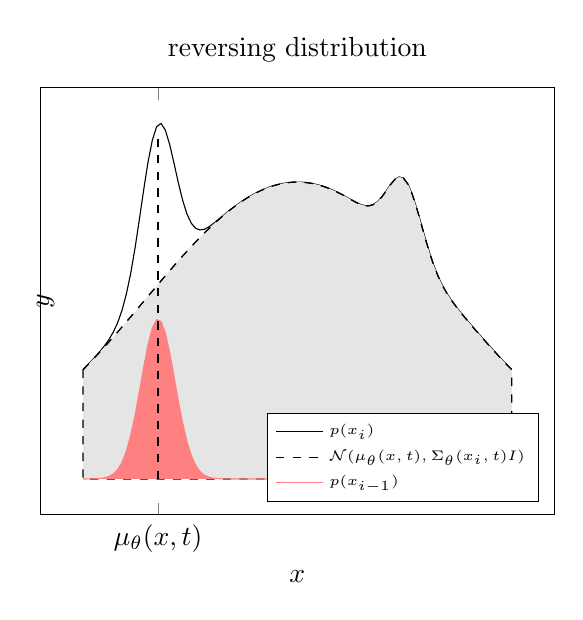
\begin{tikzpicture}
        \tikzset{
            legendmatrix/.style={% style for legends
                    draw,% draw a border for the legend
                    outer sep=.3333em,% additional space to the axis label
                    nodes={rotate=90,anchor=base west,outer sep=0pt},% rotate the nodes inside the matrix
                    /pgfplots/every crossref picture/.append style={rotate=90,yshift=.75ex}% rotate the legend images
                }}
        \begin{axis}[
                height = 7cm,
                legend style={font=\tiny,legend pos=south east,cells={anchor=west}},
                title= reversing distribution,
                axis lines = box,
                xlabel = $x$,
                ylabel = $y$,
                variable = t,
                ytick=\empty,
                xtick={-1.3},
                xticklabel={$\mu_\theta (x,t)$},
                ylabel style={at={(2ex, 0.5)}}
            ]
            \addplot [
                domain=-2:2,
                samples=100,
                color=black,
            ]
            {1.3 * exp(-x^2/4) + .3 * exp(-(x-1)^2/.05) + .7 * exp(-(x+1.3)^2/.05)};
            \addlegendentry{$p(x_i)$}
            \addplot[dashed, fill=black!10,,  domain=-2:2,samples=100] {1.3 * exp(-x^2/4) + .3 * exp(-(x-1)^2/.05)} \closedcycle;

            \addplot [
                domain=-2:2,
                samples=100,
                fill=red!50,
                color = red!50,
            ]
            { .7 * exp(-(x+1.3)^2/.05)};
            \addlegendentry{$\mathcal{N}(\mu_\theta (x,t), \Sigma_\theta (x_i,t) I)$}

            \addplot [
                dashed,
                domain=-2:2,
                samples=100,
            ]
            { 1.3 * exp(-x^2/4) + .3 * exp(-(x-1)^2/.05)};
            \addlegendentry{$p(x_{i-1})$};
            \addplot +[dashed, mark=none, color = black] coordinates {(-1.3, 0) (-1.3, 1.5)};

        \end{axis}
    \end{tikzpicture}
    we can find the parameters of the backward process just by knowing the noise level of the image, this is learned with a U-net neural network composed of a encoder and a decoder.
    By minimization of the given loss :
    \begin{equation}
        \mathcal{L} = \mathbb{E} \lVert \epsilon - \epsilon_\theta (x_i, i) \rVert ^2
        \label{eq:Loss}
    \end{equation}

    Then we can generate a new image by applying the backward process to a noise image $\epsilon \sim \mathcal{N} (0,I)$. The network will then estimate the noise level and apply the desired transformation to the image.
    which results normally in a new image with a realistic distribution of density.
    \section{Architecture}
    The architecture used in this diffusion model is a simple encoder-decoder,
    \begin{table}[H]
        \begin{small}
            \caption{layer dimensions}
            \label{tab:Size}
            \begin{center}
                \begin{tabular}[c]{l|l}
                    \hline
                    \multicolumn{1}{c|}{\textbf{Layer}} &
                    \multicolumn{1}{c}{\textbf{shape}}                                  \\
                    \hline
                    Decoder Input                       & (1, 64, 64), 2 x (10, 64, 64) \\
                    Bottlneck                           & (160, 1, 1), 2 x (160, 1, 1)  \\
                    Decoder Output                      & (20, 64,64), 2 x (10, 64,64)  \\

                    \hline
                \end{tabular}
            \end{center}
        \end{small}
    \end{table}

    \begin{figure}[H]
        \centering
        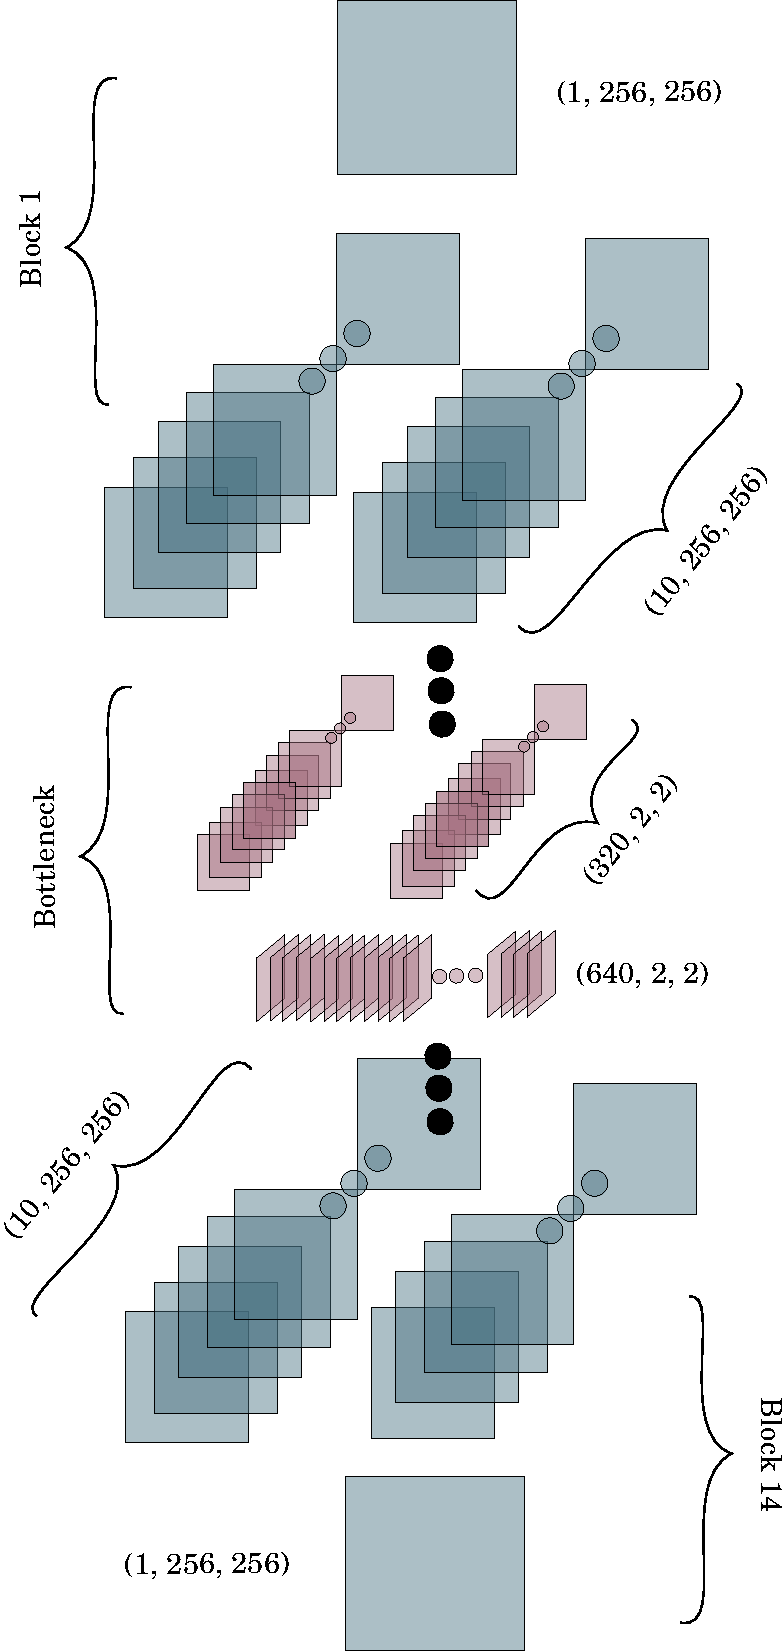
\includegraphics[width = .8\linewidth,page=1]{figure/drawing.pdf}
        \caption{Unet convolutional structure}
    \end{figure}

    \section{Testing}
    \vspace*{-1cm}

    \begin{figure}[H]
        \centering

        \begin{subfigure}[h!]{.9\linewidth}
            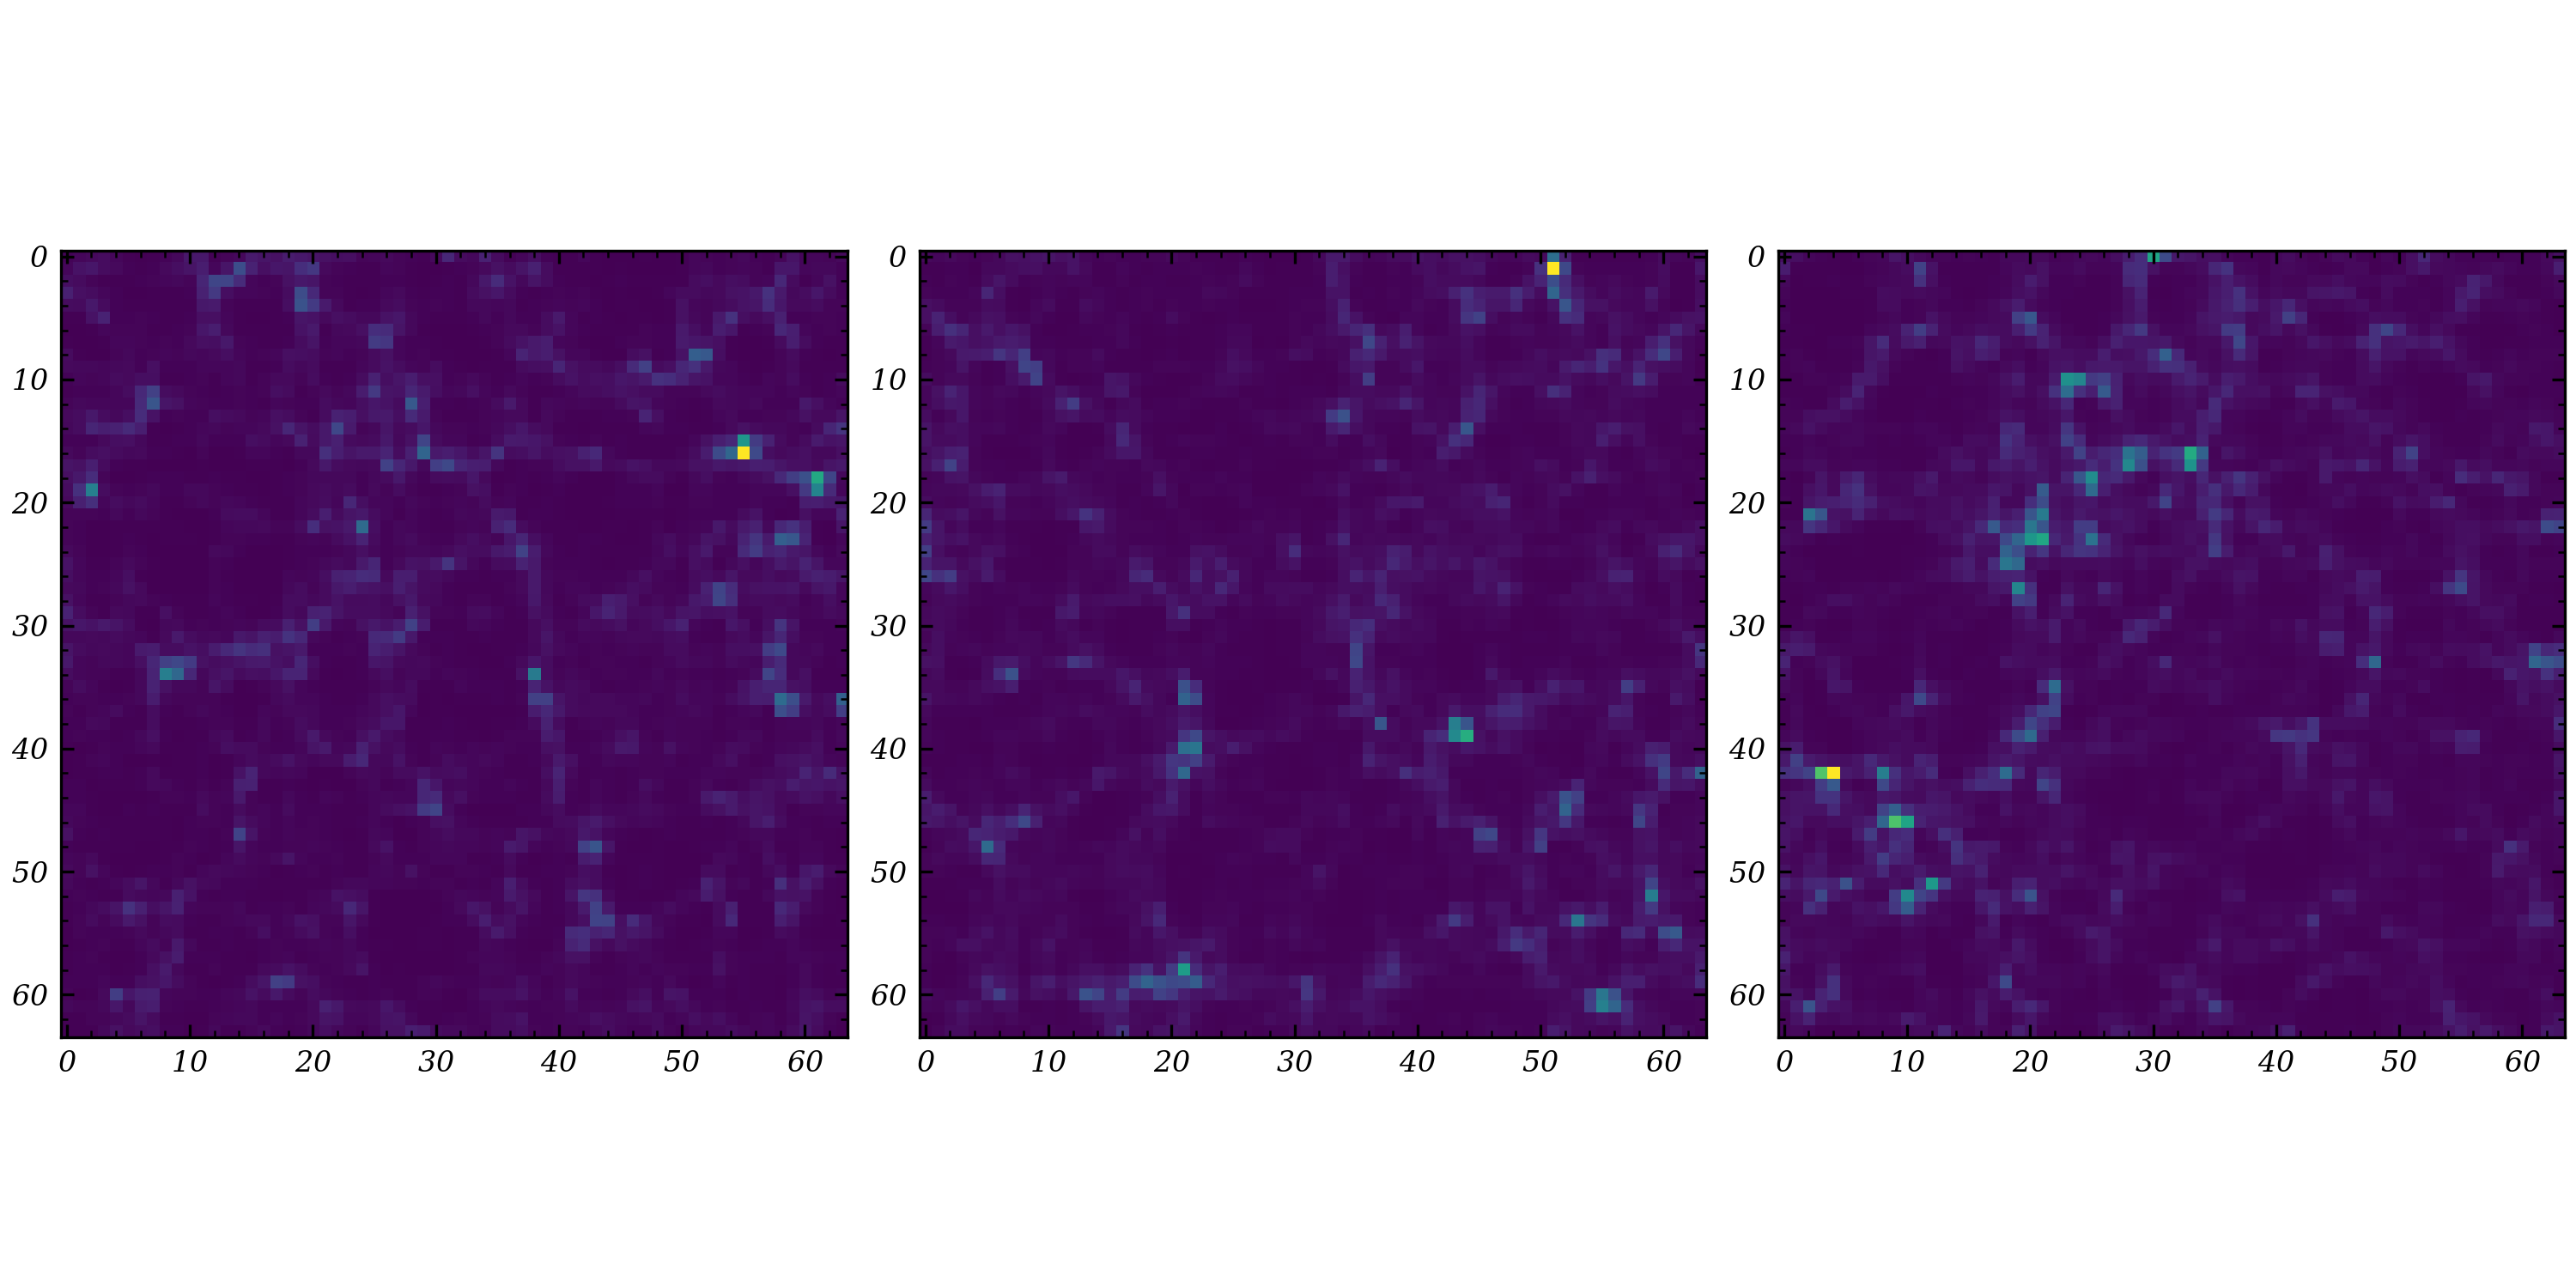
\includegraphics[width=\textwidth]{figure/training_image.png}
            \caption{Training image}
            \label{fig:training}
        \end{subfigure}
        \vfill
        \begin{subfigure}[h!]{.9\linewidth}
            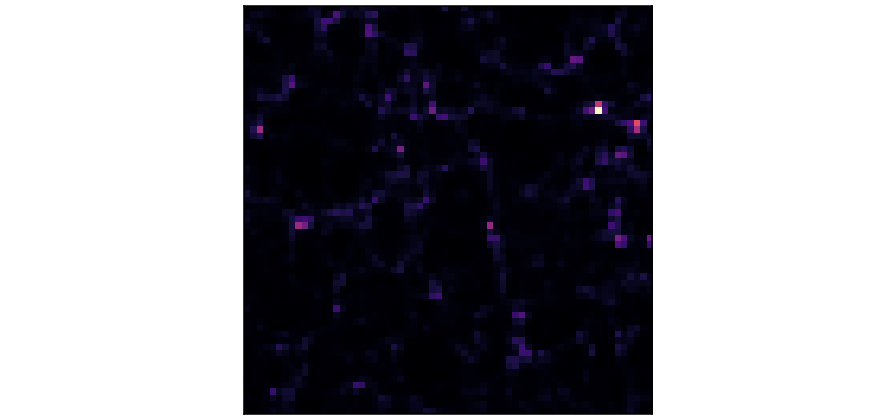
\includegraphics[width=\textwidth]{figure/generated_image.png}
            \caption{Generated image}
            \label{fig:generated}
        \end{subfigure}
        \caption{Overview of the NN data}
    \end{figure}
    The training images presents some specificities, we can clearly notice the presence of node like structures, which results from a large aggragation of galaxies. And as the priiomordial universe converged to a filamentary-like structure, the training image presents
    clear and noticeable filaments, so called "cosmic-web". In the datasets these type of struucture are also recognizable, however one clear observation is the mean value of the field which is not correct at all, \ref{fig:generated}, therefore we can just conclude as first sight that the distrubution is range relevant.
    \subsection{Loss function}
    In section 2.I we have defined the loss function as a simple difference between real noise value, and predicted one (2.1), We can then study the convergence of this loss function during the training process. for each epoch and for each batch, this gives the following graph :

    (Must retrained the NN to save this data)
    \subsection{Physics likelihood}
    \subsubsection{Histograms}

    \begin{figure}[H]
        \begin{small}
            \begin{center}
                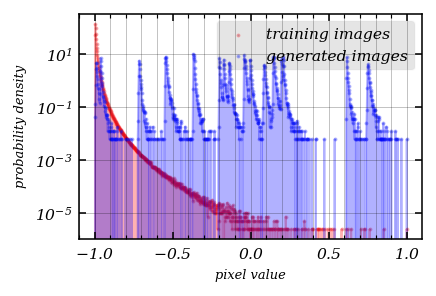
\includegraphics[width=0.95\linewidth]{figure/hist.png}
            \end{center}
            \caption{Histogran of intenties for both training and generated images, in red line the training images and in blue the generated images}
            \label{fig:hist}
        \end{small}
    \end{figure}
    Wuth \ref{fig:hist}, ze can lay the emphasis on the distribution similarity between generated and training images, however we can notice that the generated images mean values are not the same as opposed to the training images as we discussed in \textbf{2.III}. I've not find the cause of this issue \dots.

    \subsubsection{Power spectrum}

    As we discussed before, the generated images are not perfect, however besided the mean value issue, the range of the distribution seems correct. To study more precisely the characteristics of the images, one common way in astronomy is to study the power spectrum of the images. We can suppose the power spectrum isotropic in space, meaned over each y-voxel.
    The power spectrum is defined as the fourier transform of $I^2$ wuth $I$ the pixel intensity. It describes the repartition in wave vector of the power, which is not related to with the mean value of the given image, which is a good point to study the generated images.
    Here we will study the normalized power spectrum, which is defined as : [cite]

    $$P(k) = k^3 p(k)$$
    with $p(k)$ the power spectrum and $k$ the wave vector.

    \begin{figure}[H]
        \begin{small}
            \begin{center}
                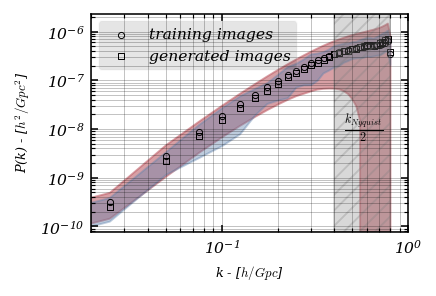
\includegraphics[width=0.95\linewidth]{figure/spectral_graph.png}
            \end{center}
            \caption{The blue fill is the standard deviation of the generated datasets, and the red one corresponds to the training image deviation. The grey shaded domain delimits the $k_{\text{nyquist}}$ validity domain, due to the descretization of space.
                The psd leads to the same conclusion, the generated images and the training image have the same power spectrum, which strengthened the previous conclusion}
            \label{fig:psd}
        \end{small}
    \end{figure}

    \begin{lstlisting}[language=Python][caption = psd code]
def compute_isotropic_psd(img : Iterable) -> tuple: 
    """
    compute_isotropic_psd compute_isotropic_psd compute isotropic power distribution of a given image

    Parameters
    ----------
    img : Iterable


        _description_

    Returns
    -------
    tuple
        tuple of Iterable (wave vector k, power vector)
    """    
    
    delta_x = 250/64
    k, p = welch(img, fs = 2 * np.pi / delta_x, axis = 0, scaling= 'spectrum', nperseg = 64)
    
    return k, np.mean(p, axis = 1)
    \end{lstlisting}

    \subsection{Third order image analysis}

    The goal of this analysis is to isolate complex structures such as filaments or nodes and to study their statistical characteristics.
    For isolating such structures, we used a graph approach, considering every pixel as a graph node connected to its nearest neighbors, this connection is removed if the pixel values is  smaller than a typical threshold value fixed by the typical deviation of the gaussian noise distribution of the primary universe.
    To find this typical length we use \emph{Fiducial} simulations at $z = 127$, which gives after renormalization process :

    $$\sigma_0 = 0.107$$


    \begin{figure}[H]
        \begin{subfigure}[b]{.48\linewidth}
            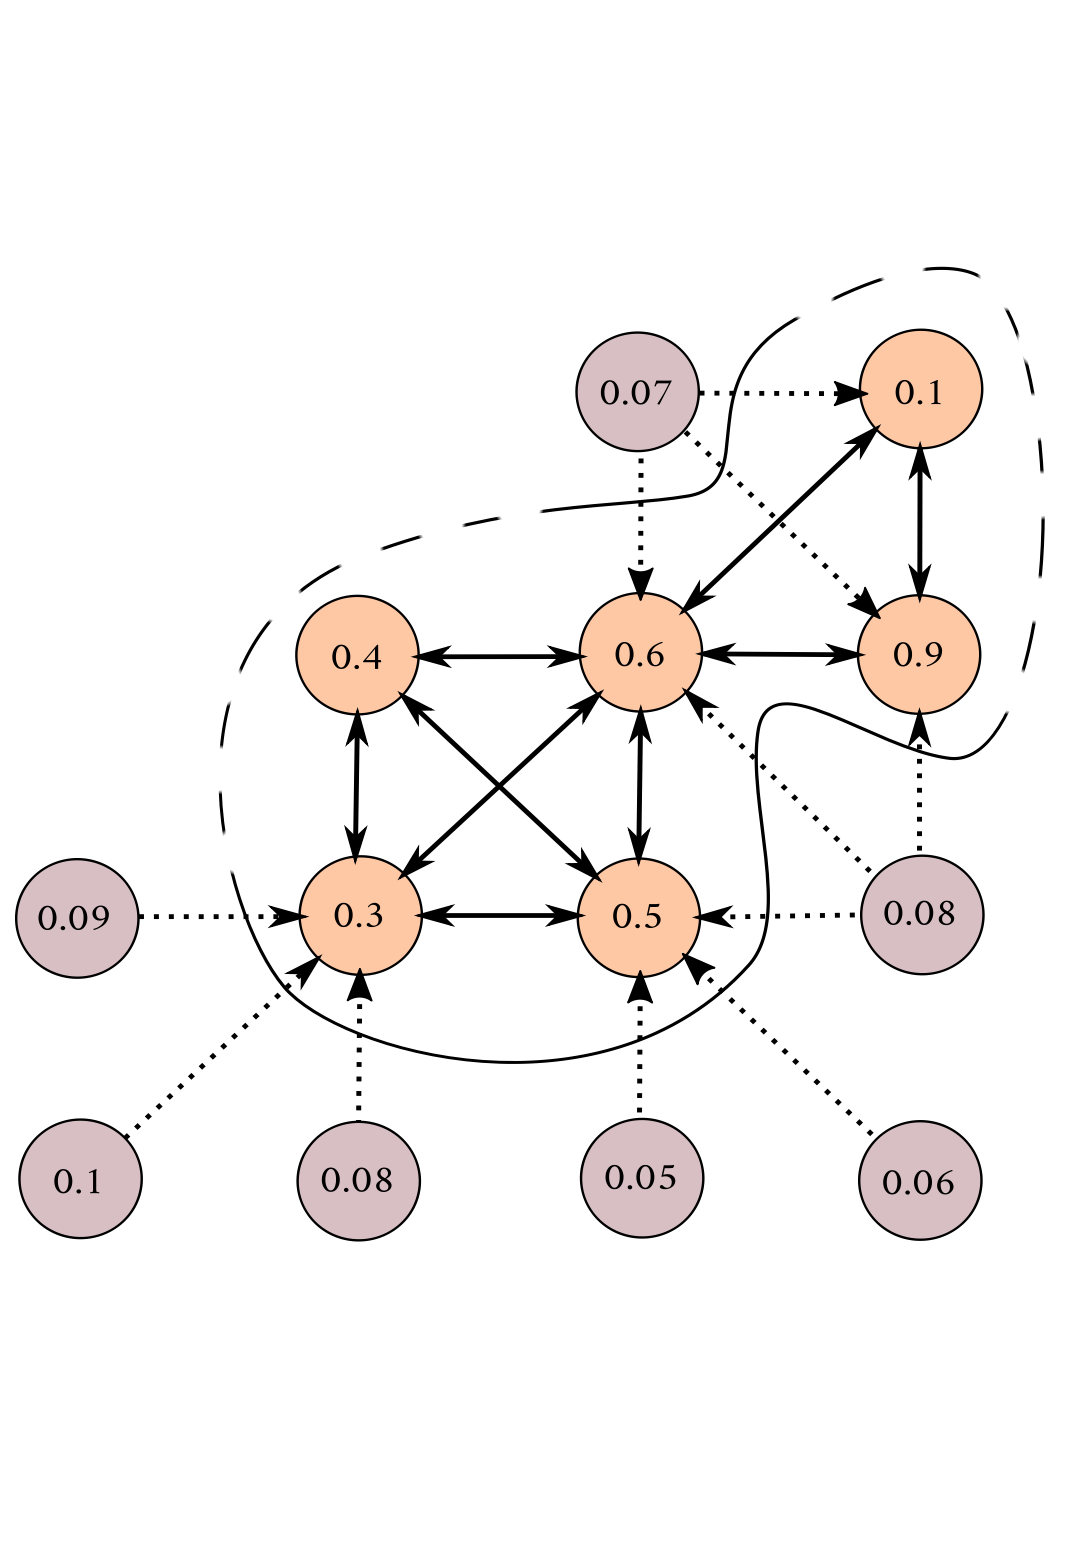
\includegraphics[width=\linewidth]{./figure/graph.png}
            \caption{Graph construction of the density field}

        \end{subfigure}
        \hfill
        \begin{subfigure}[b]{.48\linewidth}
            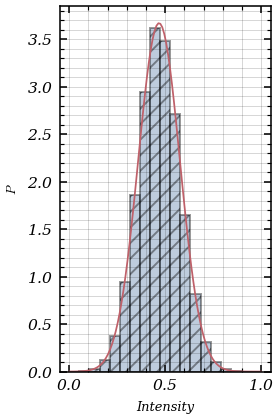
\includegraphics[width=\linewidth]{./figure/density_prim.png}
            \caption{Density distribution for $z = 127$}
        \end{subfigure}

        \caption{}
        \label{}
    \end{figure}


    \begin{figure}[H]
        \begin{subfigure}[t]{.48\linewidth}
            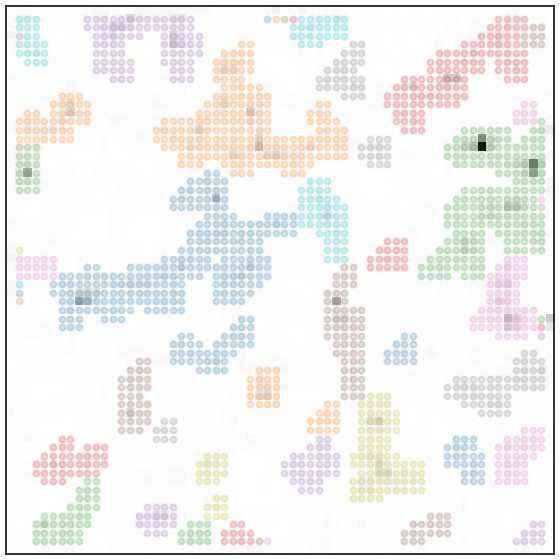
\includegraphics[width=\linewidth]{./figure/clustering_filaments.png}
            \caption{Analyzed image with many filament cluster}

        \end{subfigure}
        \hfill
        \begin{subfigure}[t]{.48\linewidth}
            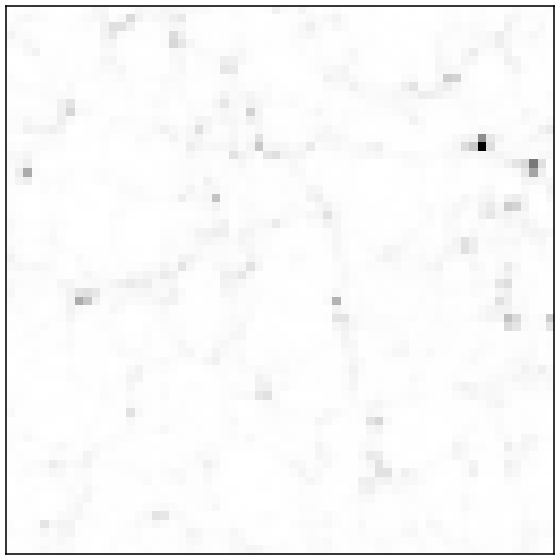
\includegraphics[width=\linewidth]{./figure/generated_image_cluster.png}
            \caption{Generated image}
        \end{subfigure}

        \caption{}
        \label{}
    \end{figure}



    \subsection{Non linear contrasting}
    To improve the contrast of previous images, a solution has been proposed by [cite], it consists of the following transformation :
    $$ \sigma : x \mapsto \frac{x}{x + a}$$
    Let's consider the number  $\mathcal{C}_{nl} = \frac{\sigma_0}{(\sqrt{a} - a)}$. The intersting point about this typical number is the following.
    If $\mathcal{C}_{nl} \ll 1 $, the contrasting functions is too weak for the filament structure, whearas for $\mathcal{C}_{nl} \gg 1$ the contrasting function is too strong for the noise. Therefore we must choose $a$, such that $\mathcal{C}_{nl} \sim 1$. The idea behind this is the following if $\mathcal{C}_{nl} \ll 1$ the derivative of the contrasting function at the typical length $\sigma_0$ is too big, it means that we do not isolate the filamentary structure. On the other hand if $\mathcal{C}_{nl} \gg 1$ the derivative of the contrasting function at the typical length $\sigma_0$ is too small, it means that we isolate the noise..
    \begin{figure}[H]
        \centering
        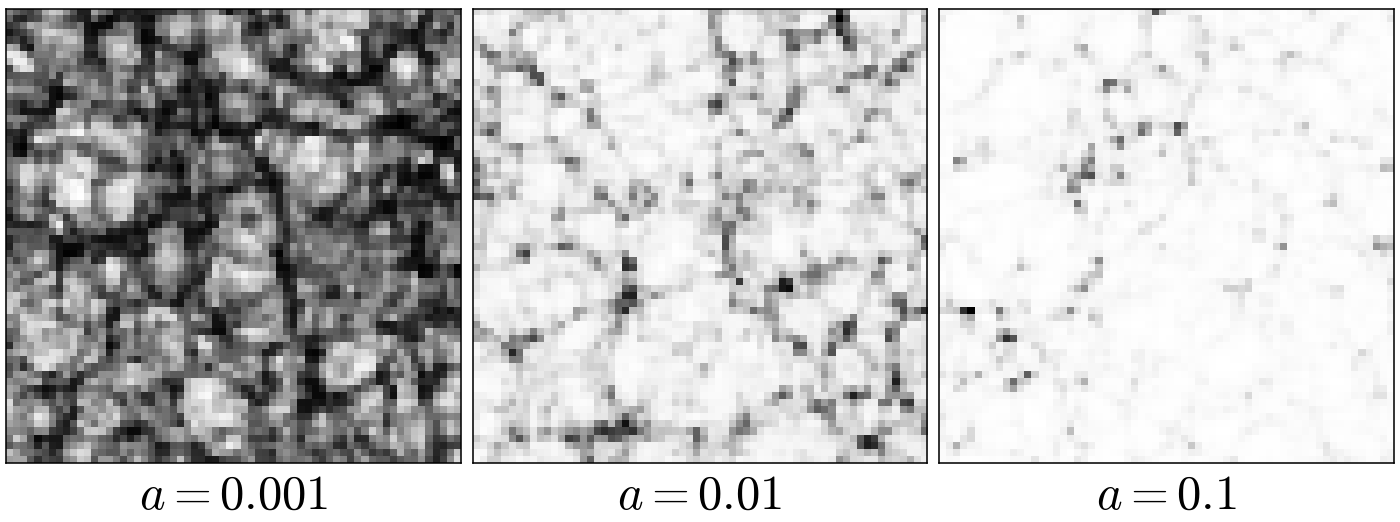
\includegraphics[width=0.99\linewidth]{./figure/img_transfo.png}
        \caption{transformations for multiple values of $a$, the extreme loglike behaviour at low $a$ is totally deforming the physics matter field. which should drastically lower the learning efficiency of the NN. For relatively high $a = 0.1$ we do nor increase a lot the filaments contrast as opposed to medium $a$ values, where the filamentary structure is clearly distinguishable, without deforming the physics field \ref{}.}
        \label{}
    \end{figure}

    \begin{figure}[H]
        \begin{subfigure}[H]{.6\linewidth}
            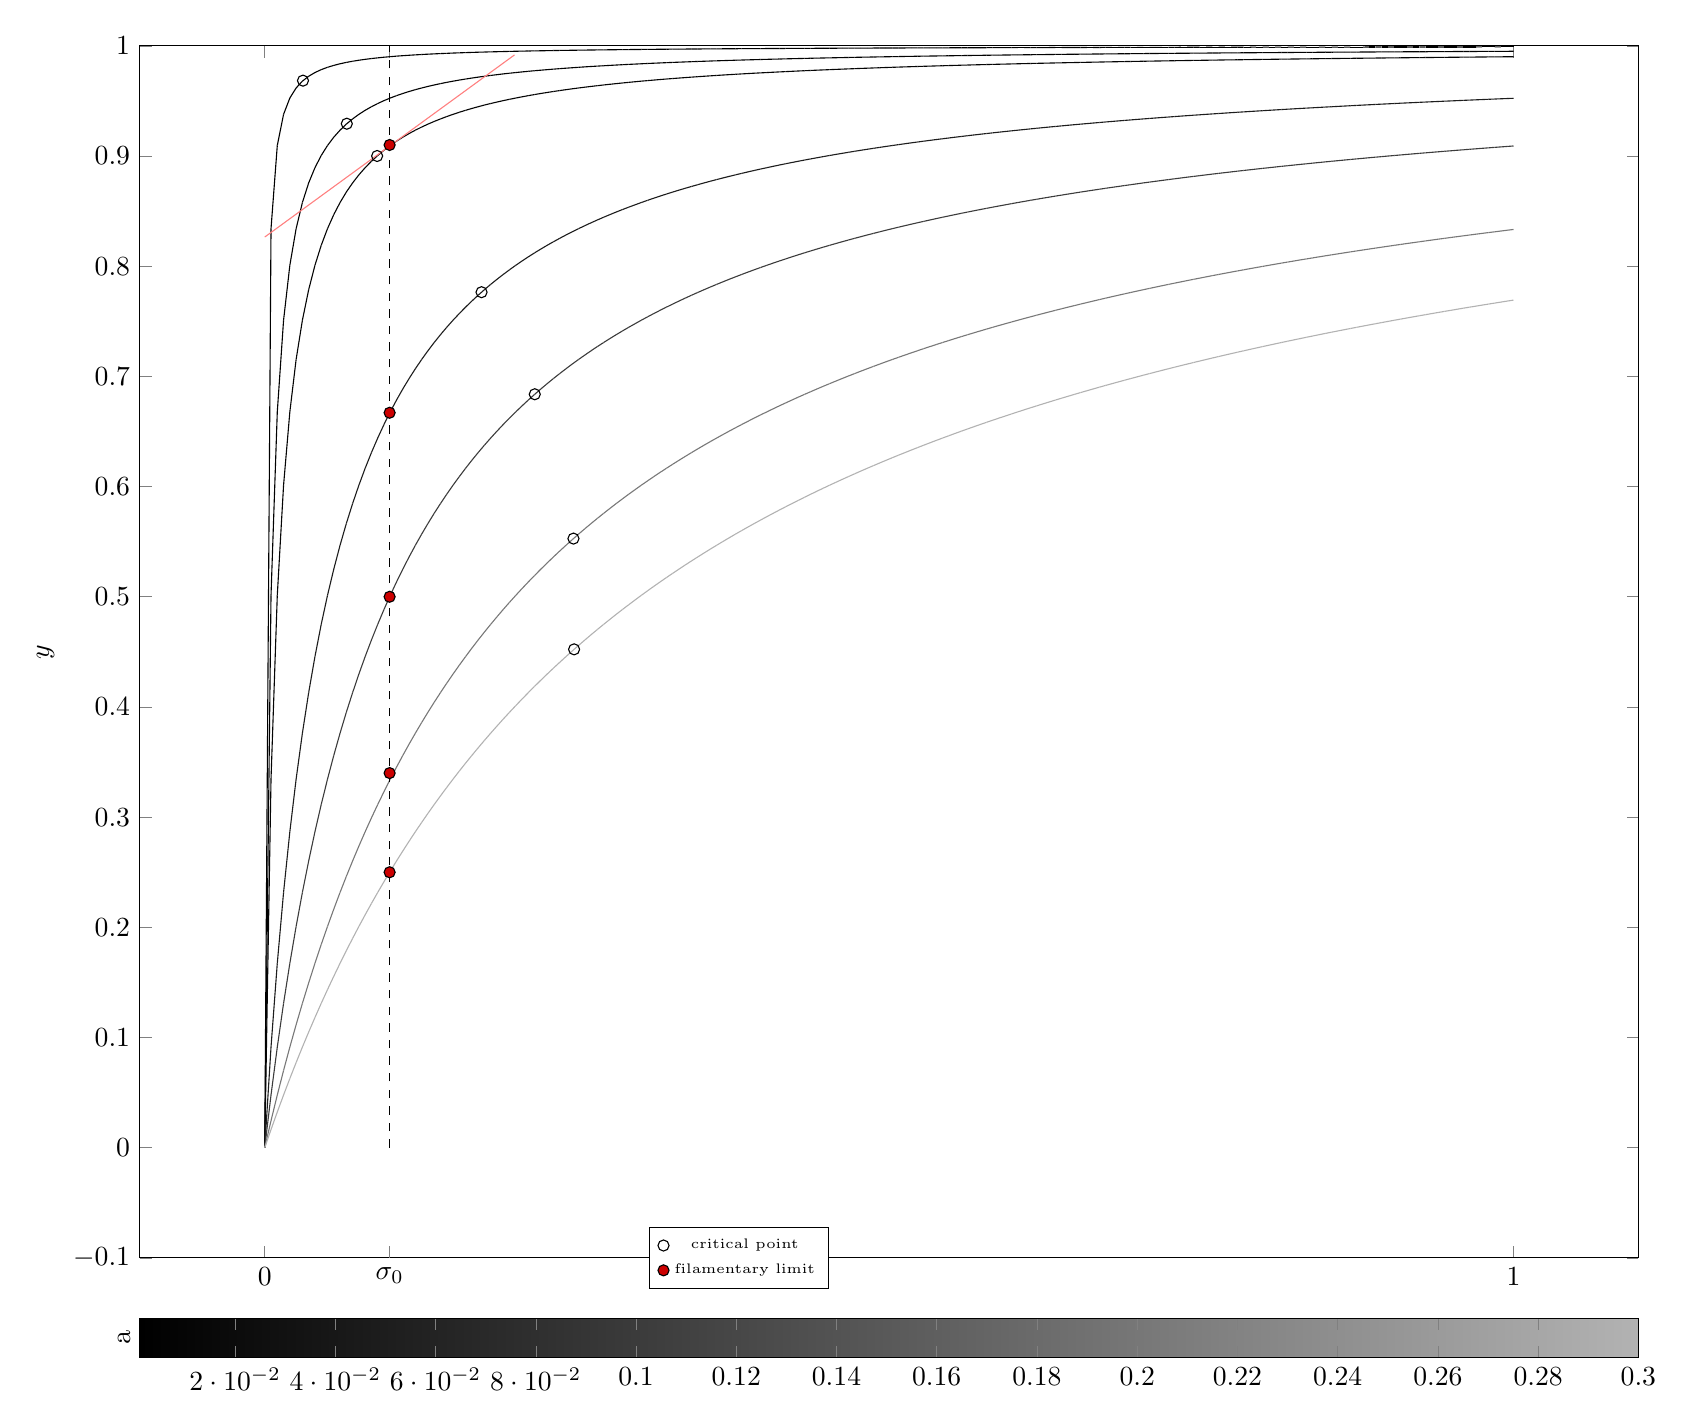
\begin{tikzpicture}
                \begin{axis}[
                        legend style={font=\tiny,at={(0.4,0.)},anchor=center},
                        axis lines = box,
                        width = 1.7\linewidth,
                        height= 1.4\linewidth,
                        ylabel = $y$,
                        variable = t,
                        trig format plots = rad,
                        colormap={blackwhite}{gray(0cm)=(0); gray(1cm)=(.7)},
                        colorbar horizontal,
                        colorbar style={ylabel = a},
                        xtick={0, 1},
                        extra x ticks={0.1},
                        extra x tick labels={$\sigma_0$},
                        ymax = 1,
                    ]
                    \foreach \a in {0.001,0.005,0.01, 0.05, 0.1, 0.2, 0.3}{
                            \edef\temp{\noexpand\addplot [mesh, point meta=\a, domain=0:1, samples=200, forget plot]{x / (x + \a)};
                            }\temp};
                    \addplot +[only marks, color = black, mark = o] coordinates {(0.03062277660168379, 0.9683772233983162)
                            (0.06571067811865475, 0.9292893218813453)
                            (0.09000000000000001, 0.9)
                            (0.17360679774997895, 0.7763932022500211)
                            (0.21622776601683794, 0.683772233983162)
                            (0.24721359549995792, 0.5527864045000421)
                            (0.24772255750516609, 0.4522774424948339)};
                    \addlegendentry{critical point};
                    \addplot +[only marks, color = black, mark = *] coordinates {(0.1, 0.91) (0.1,0.667) (0.1, 0.5) (0.1, 0.34)  (0.1, 0.25)};
                    \addlegendentry{filamentary limit};
                    \addplot +[dashed, mark=none, color = black] coordinates {(0.1, 0) (0.1,1)};
                    \foreach \a in {0.01}{
                            \edef\temp{\noexpand\addplot [domain=0:0.2, samples=100,color = red!50]{\a / (0.1 + \a)^2 * (x - 0.1) + 0.1 / (0.1 + \a)};
                            }\temp};
                \end{axis}
            \end{tikzpicture}
            \caption{Analyzed image with many filament cluster}
            \label{fig:clustering}

        \end{subfigure}
        \hfill
        \begin{subfigure}[H]{.35\linewidth}
            \vspace{-1.5cm}
            \caption{}
            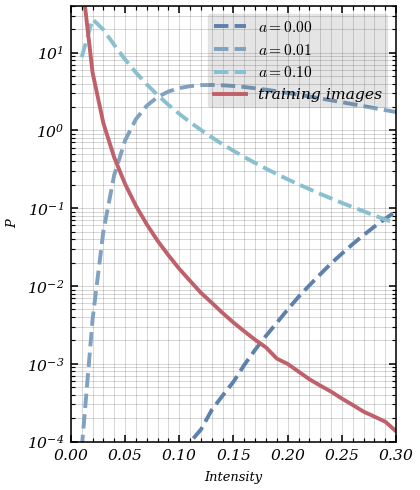
\includegraphics[width=\linewidth]{./figure/distr_transfo.png}
            \label{fig:density}
        \end{subfigure}

        \caption{In the Contrast transformations where the parameter $a$ is chosen to optimize the contrats given the previous normalization process. These functions allow us to shrink the inage domain after a critical value (\ref{fig:clustering}), which should be choosen accordingly to threshold used in the clustering process.
            Indeed we wanna isolate the filamentary structures from the noisy background, which is not too small, otherwise we will isolate the noise, and not too big, otherwise we will not isolate the filaments. Given \ref{fig:density} we can observe the migration of intensity distribution for low $a$, it means that a lot of noisy pixel have been strenghtened, which is not what we want. For relatively high $a  \sim 0.3$ we do ont isoliate the filaments anymore, because the crticial intensity is much higher}
        \label{}

    \end{figure}

    \chapter{GAN neural Network}

    \section{Theoretical background}

    \begin{enumerate}
        \item G generates 32 images from 32 sets of 100 random numbers
        \item D discriminates the images from the
              32 real images (labelled 1) and the 32 images generated by G (labelled 0)
        \item D learns from its mistakes
        \item G generates 32 images from 32 sets of 100 new random numbers
        \item D gives probabilities for the 32 generated images
        \item G learns from the mistakes of D
        \item we plot 16 generated images from 16 * 100 new random numbers to see if G always generates the same images
        \item we plot a generated image and a real image to compare them
        \item we print the outputs of the loss functions for this epoch
    \end{enumerate}

    \section{Architecture}


    \begin{lstlisting}[language=Python, caption=Python example]
class Discriminator(nn.Module):
    def __init__(self):
        self.model = nn.Sequential(
            nn.Linear(4096, 2048),      # 64x64 input image 
                                        # = 4096 pixels
            nn.ReLU(),
            nn.Dropout(.3),
            nn.Linear(2048, 1024),
            nn.ReLU(),
            nn.Dropout(.3),
            nn.Linear(1024, 512),
            nn.ReLU(),
            nn.Dropout(.3),
            nn.Linear(512, 256),
            nn.ReLU(),
            nn.Dropout(.3),
            nn.Linear(256, 1),
            nn.Sigmoid(),               # Discriminator gives a 
                                            # probability as output          
            )
            
    def forward(self, x):
        x = x.view(x.size(0), 4096)     # Vectorization
        output = self.model(x)
        return output
    \end{lstlisting}

    Training the model
    \lstinputlisting[language=Python]{./codes/train_gan.py}

    \section{Testing}

    \begin{center} \rule{.5\linewidth}{1pt} \end{center}

    \subsection{Results}
    After 10 epochs (15 min):
    \begin{figure}[H]
        \centering
        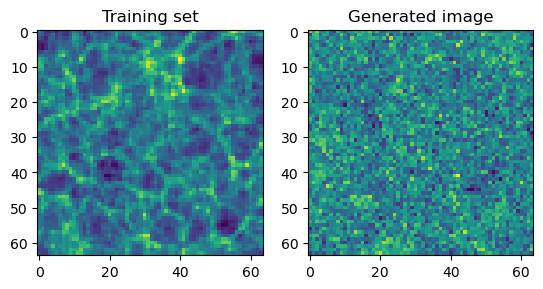
\includegraphics[width = .9\linewidth]{./figure/10epochs_32batch.png}
    \end{figure}
    \begin{figure}[H]
        \centering
        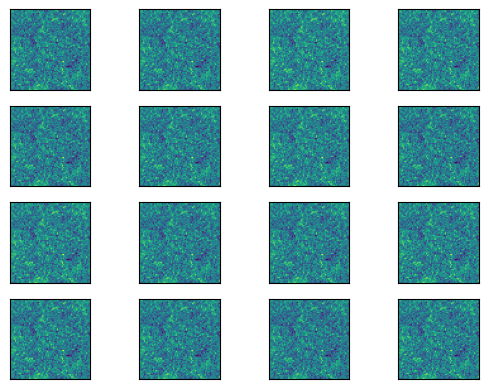
\includegraphics[width = .9\linewidth]{./figure/10epochs_32batch_queblo.png}
    \end{figure}

    After 100 epochs (one night):
    \begin{figure}[H]
        \centering
        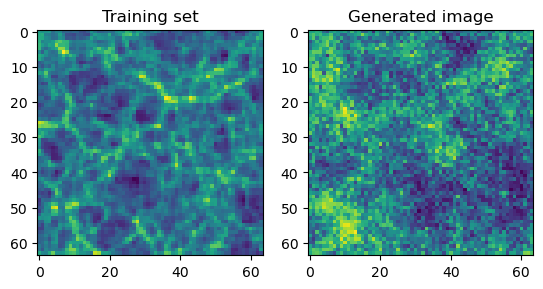
\includegraphics[width = .9\linewidth]{./figure/100epochs_32batch.png}
    \end{figure}
    \begin{figure}[H]
        \centering
        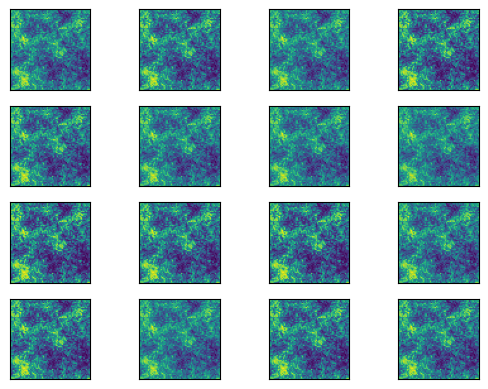
\includegraphics[width = .9\linewidth]{./figure/100epochs_32batch_queblo.png}
    \end{figure}



    \begin{itemize}
        \item Visually, the ouput of the generator does not seem to depend on its input as show the 16 very similar images produced by different inputs for epochs 10 and 100.
        \item D and G are trained on a 32 size dataset. If we want to use the whole dataset, then I have to choose between either loading the whole dataset in the train loader but then I improve D and G every 3 hours, or  picking 32 new images at random for every epoch but then it's not an epoch anymore, and additionally my computer has a tendency to crash.
        \item Need for a statistical tool to analyse the images.
    \end{itemize}

    \subsection{Loss function}

    \subsection{Physics likelihood}
    \subsubsection{Histograms}
    \subsubsection{Power spectrum}

    \chapter{Discussions}


\end{multicols*}
\end{document}